\documentclass[12pt]{article}
\setlength{\parindent}{0pt}

\usepackage{tikz}
\usetikzlibrary{arrows.meta}
\usepackage{float}

\usepackage{mathpazo}

\usepackage{hyperref}
\hypersetup{
    colorlinks=true,
    linkcolor=blue,
    filecolor=magenta,
    urlcolor=cyan}
\urlstyle{same}

\title{Mikami's Mistake (not again?!)}
\date{}

\begin{document}

\maketitle

\section*{Problem Statement}

In a parallel universe, \href{https://deathnote.fandom.com/wiki/Light_Yagami}{Light Yagami} realizes he can no longer rely on \href{https://deathnote.fandom.com/wiki/Kiyomi_Takada}{Kiyomi Takada} (beauty without brain??) to discreetly relay his judgments to \href{https://deathnote.fandom.com/wiki/Teru_Mikami}{Teru Mikami}. Instead, he decides to send his encrypted instructions as a discrete-time signal sequence,  $x[n]=[a,b,c,d]$.\\

To decode the message, Mikami is instructed to build a dedicated hardware module to compute the standard \textbf{4-point Fast Fourier Transform (FFT)} of the signal. However, in his zealous haste, Mikami makes a critical engineering error. He wires the FFT machine using a standard \textbf{Decimation-in-Frequency (DIF)} structure — meaning the inputs $x[0]$ to $x[3]$ enter in normal order, twiddle factors are applied in the first stage, and the final outputs are read in bit-reversed order.\\

The fatal flaw lies in the Arithmetic Logic Units (ALUs). Mikami mistakenly programs them to execute \textbf{Decimation-in-Time (DIT)} butterfly formulas. Instead of calculating the sum and difference \emph{first} and then multiplying the difference by the twiddle factor $W_4^k$, Mikami’s corrupted machine multiplies the bottom branch by $W_4^k$ before evaluating the sum and difference.

\begin{figure}[H]
\centering

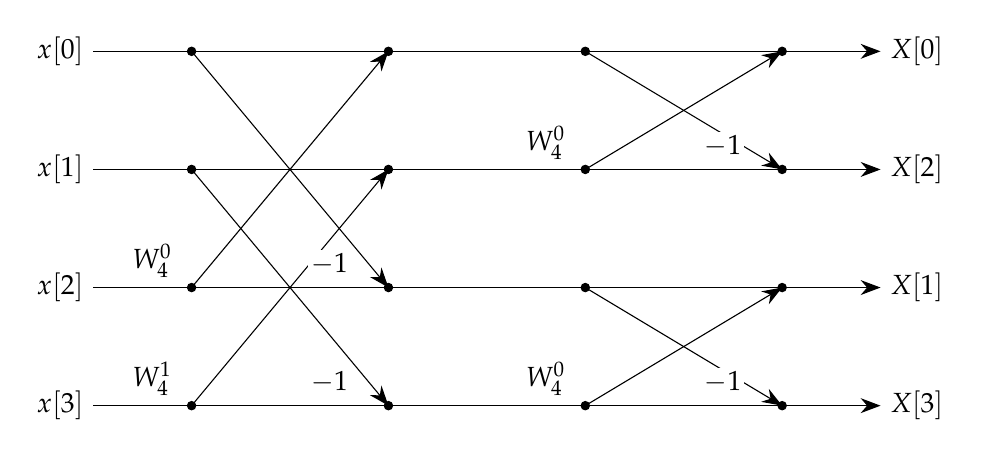
\begin{tikzpicture}[>={Stealth[scale=1.5]}, x=2.5cm, y=-1.5cm]
    \node[left] at (0,0) {$x[0]$};
    \node[left] at (0,1) {$x[1]$};
    \node[left] at (0,2) {$x[2]$};
    \node[left] at (0,3) {$x[3]$};
    

    \node[right] at (4,0) {$X[0]$};
    \node[right] at (4,1) {$X[2]$};
    \node[right] at (4,2) {$X[1]$};
    \node[right] at (4,3) {$X[3]$};

    
    \draw[->] (0,0) -- (4,0);
    \draw[->] (0,1) -- (4,1);
    \draw[->] (0,2) -- (4,2);
    \draw[->] (0,3) -- (4,3);
    

    \draw[->] (0.5, 0) -- (1.5, 2);
    \draw[->] (0.5, 1) -- (1.5, 3);
    \draw[->] (0.5, 2) -- (1.5, 0);
    \draw[->] (0.5, 3) -- (1.5, 1);

    
    \node[fill=white, inner sep=1pt] at (1.2, 1.8) {$-1$};
    \node[fill=white, inner sep=1pt] at (1.2, 2.8) {$-1$};
    

    \node[above] at (0.3, 2) {$W_4^0$};
    \node[above] at (0.3, 3) {$W_4^1$};
    

    \draw[->] (2.5, 0) -- (3.5, 1);
    \draw[->] (2.5, 2) -- (3.5, 3);
    \draw[->] (2.5, 1) -- (3.5, 0);
    \draw[->] (2.5, 3) -- (3.5, 2);
    

    \node[fill=white, inner sep=1pt] at (3.2, 0.8) {$-1$};
    \node[fill=white, inner sep=1pt] at (3.2, 2.8) {$-1$};
    
    
    \node[above] at (2.3, 1) {$W_4^0$};
    \node[above] at (2.3, 3) {$W_4^0$};
    

    \foreach \x in {0.5, 1.5, 2.5, 3.5} {
        \foreach \y in {0, 1, 2, 3} {
            \filldraw (\x,\y) circle (1.5pt);
        }
    }
\end{tikzpicture}

\caption{Mikami's 4-point Fast Fourier Transform}
\end{figure}

Upon realizing his fatal mistake, Mikami clutches his head, frantically staring at the useless hardware, and cries out, \emph{``\href{https://en.wikipedia.org/wiki/Kami}{Kami}! Forgive my insolence! I have failed to execute your will! Please tell me what to do!''}\\

Mercifully, Light hears his devout follower's plea, but he needs your help. You are a brilliant mathematician and Light's secret confidant. Since Mikami's hardware is permanently fused and cannot be physically rewired, Light wishes to bypass the defect mathematically. He asks you to develop an algorithm that takes his originally intended sequence $x[n]$ and transforms it into a pre-conditioned signal $x'[n]$. When Mikami feeds $x'[n]$ instead of $x[n]$ into his corrupted machine, the hardware mathematically corrects itself, outputting the exact, correct FFT spectrum of the original sequence $x[n]$. Only then can Mikami decode the message and proceed with the judgment.\\

You must derive the expressions for $x'[n]$ in terms of $a, b, c, d$. \textbf{Do it fast, because \href{https://deathnote.fandom.com/wiki/Near}{Near} is near!}

\end{document}